  % vim: set ts=4 sw=4 ai et tw=74:
\documentclass[12pt,a4paper,portuges]{style/myreport}
\usepackage[portuges]{babel}
\usepackage[utf8]{inputenc}

%%%%%%%%%%%%%%%%%%%%%%%%%%%%%%%%%%%%% DADOS DA CAPA DO RELATÓRIO %%%%%%%%%%%%%%%%%%%%%%%%%%%%%%%%%%%%%%5
\newcommand{\AnoLectivo}{Ano Lectivo de 2010/11}
\newcommand{\TituloProjecto}{Planeta XPTO, Fase Final}
\newcommand{\NomeDaCadeira}{Disciplina de Computação Gráfica}
\newcommand{\Curso}{Licenciatura em Engenharia Informática}

\newcommand{\PrimeiraListaNomes}{António Cascais, Fábio Costa, Gabriel Poça, José Teixeira, Miguel Palhas}

\newcommand{\PrimeiroElemento}{54744 - António Carlos Pinheiro Cascais}
\newcommand{\SegundoElemento}{54822 - Fábio Rafael Costa}
\newcommand{\TerceiroElemento}{56974 - Gabriel Gonçalves Poça}
\newcommand{\QuartoElemento}{54749 - José António Teixeira}
\newcommand{\QuintoElemento}{54767 - Miguel Branco Palhas}
%%%%%%%%%%%%%%%%%%%%%%%%%%%%%%%%%%%%% FIM %%%%%%%%%%%%%%%%%%%%%%%%%%%%%%%%%%%%%%5

\usepackage[T1]{fontenc}
\usepackage{a4wide}
\usepackage{txfonts}% use Arial && Times New Roman
\usepackage[pdftex]{color,graphicx}
\usepackage{fancyhdr}
\usepackage{fancyvrb}
\usepackage{acronym}
\usepackage{cite}
\usepackage{longtable}
\usepackage{datetime}
%\usepackage{amssymb}
\usepackage[pdfauthor={\PrimeiraListaNomes},%
            pdftitle={\{\TituloProjecto\}},%
            urlcolor=darkblue,%
            citecolor=darkblue,%
            filecolor=darkblue,%
            linkcolor=darkblue,%
            pdftex,colorlinks,a4paper]{hyperref}
\definecolor{darkblue}{rgb}{0,0,0.6}
%\definecolor{darkred}{rgb}{0.8,0,0}

%%%%%%%%%%%%%%%%%%%%%%%%%%%%%%%%%%%% PACOTES PARA ADICIONAR CODIGO FONTE %%%%%%%%%%%%%%%%%%%%%%%%%%%%%%%%%%%%%%
\usepackage{listings}
\usepackage{color}
\usepackage{textcomp}
\definecolor{listinggray}{gray}{0.9}
\definecolor{lbcolor}{rgb}{0.9,0.9,0.9}
\lstset{
	%backgroundcolor=\color{lbcolor},   					% COR DE FUNDO
	tabsize=4,
	rulecolor=,
	language=c,								% TIPO DE LINUGAGEM DE PROGRAMAÇÃO
        basicstyle=\scriptsize,
        upquote=true,
        aboveskip={1.5\baselineskip},
        columns=fixed,
        showstringspaces=false,
        extendedchars=true,
        breaklines=true,
        prebreak = \raisebox{0ex}[0ex][0ex]{\ensuremath{\hookleftarrow}},
        %frame=single,								% LINHA QUE CONTORNA O CODIGO
        showtabs=false,
        showspaces=false,
        showstringspaces=false,
        identifierstyle=\ttfamily,
        keywordstyle=\color[rgb]{0,0,1},
        commentstyle=\color[rgb]{0.133,0.545,0.133},
        stringstyle=\color[rgb]{0.627,0.126,0.941},
}

%%%%%%%%%%%%%%%%%         UTILIZAÇÃO:
%%%%%%%%%%%%
%%%%%%%%%%                  Imprimir com uma linha à volta do código
%%%%%%%%%%                       \begin{lstlisting}[frame=single]
%%%%%%%%%%
%%%%%%%%%%                  Imprimir normalmente:
%%%%%%%%%%                       \begin{lstlisting}
%%%%%%%%%%                           #include <SDL.h>
%%%%%%%%%%                       \end{lstlisting}
%%%%%%%%%%
%%%%%%%%%%                  Imprimir Ficheiro:
%%%%%%%%%%                       \lstinputlisting{filename.java}
%%%%%%%%%%%%
%%%%%%%%%%%%%%%%%%%%%%%%%%%%%%%%%%%% FIM %%%%%%%%%%%%%%%%%%%%%%%%%%%%%%%%%%%%%%

%%%%%%%%%%%%%%%%%%%%%%%%%%%%%%%%%%%% COMO ADICIONAR IMAGENS NO RELATÓRIO %%%%%%%%%%%%%%%%%%%%%%%%%%%%%%%%%%%%%%
%%%%%%%%%%%%%%
%                 \begin{figure}[here]
%                 \centering{\includegraphics[width=0.5\textwidth]{images/1imagem.png}}
%                 \caption{Prototipo de imagem}
%                 \label{fig:prototype}
%                 \end{figure}
%
%                 Please see Figure ~\ref{fig:prototype} for a prototype blah blah blah
%%%%%%%%%%%%%%
%%%%%%%%%%%%%%%%%%%%%%%%%%%%%%%%%%%% FIM %%%%%%%%%%%%%%%%%%%%%%%%%%%%%%%%%%%%%%

\pdfpagewidth=\paperwidth
\pdfpageheight=\paperheight

\renewcommand\familydefault{\sfdefault}% usar font sem serifas


%%%%%%%%%%%%%%%%%%%%%%%%%%%%%%%%%%%%% HEADER das paginas %%%%%%%%%%%%%%%%%%%%%%%%%
\pagestyle{fancy}

\fancyhead[LO,RE]{\footnotesize \slshape \rightmark}
\fancyhead[LE,RO]{\footnotesize \slshape \leftmark} 
%\fancyfoot{}
%\fancyfoot[LO,RE]{\thepage}

%%%%%%%%%%%%%%%%%%%%%%%%%%%%%%%%%%%% FIM %%%%%%%%%%%%%%%%%%%%%%%%%%%%%%%%%%%%%%

% definir acrónimos com itálico
%\renewcommand*{\acf}[1]{\acffont{\textit{\acl{#1}}~\acfsfont{(\acs{#1})}}}

\newtheorem{defin}{Definição}

%\pagestyle{fancy}
%\lhead{}
%\rhead{}

\newenvironment{comando}
{\medskip
\begin{tt}}
{\end{tt}
\medskip}

\parindent=0pt
\parskip=4pt

%
% Commands and environments
%
%% vim: set ts=4 sw=4 ai et:

% insere uma imagem com legenda, por omissao com 12cm de largura
\newcommand{\image}[3][12cm]
{
    \begin{figure}[!h]
        \begin{center}
            \includegraphics[width=#1]{images/#2}
                \caption{#3}
                \label{fig:#2}
        \end{center}
    \end{figure}
    % force dump image queue here
    %\clearpage
}


\begin{document}

%% Capa Principal %%%%%%%%%%%%%%%%%%%%%%%%%%%%%%%%%%%%%%%%%%%%%%%%%%%%%%%
\thispagestyle{empty}

\setlength{\unitlength}{1cm}
\begin{picture}(0,0)

\put(14,0){\line(0,-1){24.5}}
\put(0,-12.2){\line(1,0){18}}
\put(0,-16.2){\line(1,0){18}}
\put(0,-12.2){\line(0,-1){4}}

\put(14.5,-3){
\includegraphics[height=2cm]{style/images/um}}
\put(14.5,-6){
\includegraphics[height=2cm]{style/images/eng}}
\put(14.5,-9){
\includegraphics[height=2cm]{style/images/di}}

\begin{minipage}[t]{16cm}
 
~

\addvspace{4cm}

Universidade do Minho

Conselho de Cursos de Engenharia

\Curso

\bigskip

{\Large \textbf{\NomeDaCadeira}}

\medskip

\AnoLectivo

\addvspace{7cm}

{\LARGE \ \TituloProjecto}

\addvspace{2.5cm}

\textbf{\PrimeiraListaNomes}

Grupo 26

\addvspace{0.5cm}

%
% Supervisão:  {\textless}{\textless}Orientador{\textgreater}{\textgreater}

\addvspace{2.5cm}

{\large \monthname, \newdateformat{dashdat}{\THEYEAR} \dashdat\today}

\end{minipage}
\end{picture}

\newpage

%% Segunda página %%%%%%%%%%%%%%%%%%%%%%%%%%%%%%%%%%%%%%%%%%%%%%%%%%%%%%%
\thispagestyle{empty}

\begin{flushright}
\begin{tabular}{|p{4cm}|p{4cm}|}
\hline
Data de Recepção & \\
\hline
Responsável & \\
\hline
Avaliação & \\
\hline
Observações & \\
& \\
& \\
\hline
\end{tabular}
\end{flushright}

~

\addvspace{8.4cm}

{\LARGE \textbf{ \TituloProjecto }}

\addvspace{2.5cm}

\textbf{\PrimeiroElemento}

\bigskip

\textbf{\SegundoElemento}

\bigskip

\textbf{\TerceiroElemento}

\bigskip

\textbf{\QuartoElemento}

\bigskip

\textbf{\QuintoElemento}

\addvspace{1.5cm}

{\large \monthname, \newdateformat{dashdate}{\THEYEAR} \dashdate\today}

\newpage

%% Página de dedicatória (opcional) %%%%%%%%%%%%%%%%%%%%%%%%%%%%%%%%%%%%%
%\thispagestyle{empty}

%{\textless}{\textless}Dedicatória{\textgreater}{\textgreater}

%\newpage

%% Resumo e Índices %%%%%%%%%%%%%%%%%%%%%%%%%%%%%%%%%%%%%%%%%%%%%%%%%%%%%
\pagenumbering{roman}
% vim: set ts=4 sw=4 ai et tw=74:
\chapter*{Resumo}
\addcontentsline{toc}{chapter}{Resumo} 


% indices
%\renewcommand{\contentsname}{Índice}
\tableofcontents
\addcontentsline{toc}{chapter}{\contentsname}

%\renewcommand{\listfigurename}{Índice de Figuras}
\listoffigures
\addcontentsline{toc}{section}{\listfigurename}

%%%%%%%%%%%%%%%%%%%%%%%%%%%%%%%%%%%% LISTA DE TABELAS %%%%%%%%%%%%%%%%%%%%%%%%%%%%%%%%
%\renewcommand{\listtablename}{Índice de Tabelas}
%\listoftables
%\addcontentsline{toc}{section}{\listtablename}

\newpage

%% Texto normal %%%%%%%%%%%%%%%%%%%%%%%%%%%%%%%%%%%%%%%%%%%%%%%%%%%%%%%%%
\pagenumbering{arabic}

%% TODO: uncomment chapters

À descoberta, digamos que esse foi o lema de todo o desenvolvimento, desde os requisitos obrigatórios aos extras, como o skybox, o salto, as animações, etc. Terminamos com algo cuja imagem fala por si, o jogo é simples, aos requisitos acrescentamos as árvores, de referir também as colisões com árvores e torres, a possibilidade de saltar, e assim evitar as balas, o céu, as animações, as imagem das vidas, o full screen, isto.
A de implementação contamos com o documento de configuração \textit{.ini}, o md2loader, profilling, entre outros.


\newpage	

\chapter{Mapa de alturas e navegação}

\chapter{Disparos}
\newpage
\chapter{View Frsutum Culling}

Da teoria à prática, a maior dificuldade. De entre as diferentes abordagens, após alguma pesquisa, ficamos pela {\bf Geométrica}, pelo simples facto de não existir desvantagens notáveis face às restantes. Deste modo o View Frustum Culling está implementado para balas, torres e árvores.

\section{Bounding Spheres}
Está claro que \textit{axis aligned bounding boxes} é uma melhor implementação que \textit{bounding spheres} uma vez que permite criar uma menor margem de erro para casos de objectos no limite do frustum. No entanto trata-se de um jogo com poucos objectos onde a diferente margem de erro não será significativa e como tal \textit{bounding spheres} são a melhor escolha vez que apresentam o mesmo resultado e mais facil implementação.


\begin{lstlisting}[caption=Método para teste com \textit{bounding spheres}.]
int Frustum::sphereInFrustum(Vertex *p, float raio) {

    int result = INSIDE;
    float distance;

    for (int i = 0; i < 6; i++) {
        distance = pl[i].distance(p);
        if (distance < -raio)
            return OUTSIDE;
        else if (distance < raio)
            result = INTERSECT;
    }
    return (result);

}
\end{lstlisting}

\begin{figure}[here]
                 \centering{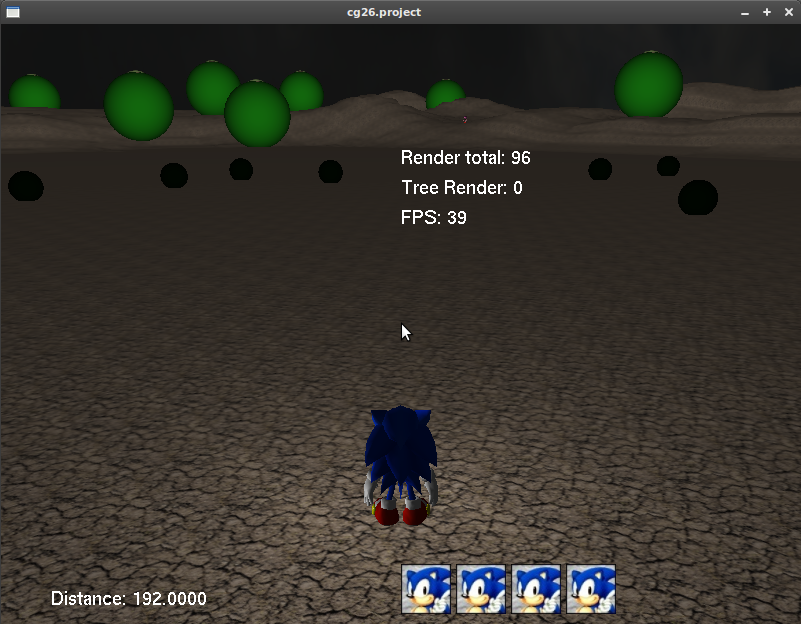
\includegraphics[width=0.8\textwidth]{images/frustum.png}}
                 \caption{Implementação de \textit{bounding spheres}.}
                 \label{fig:prototype}
\end{figure}
\newpage
\chapter{Profiling}
Ainda que um extra, ou talvez mesmo não um extra uma vez que é uma componente de desenvolvimento não de jogo, cramos também um modulo para profiling. Para efectuar os calculos existem três arrays para guardar a informação:

\begin{description}
\item[\textit{start}] Registo o tempo no inicio da medição.
\item[\textit{end}] Regista o tempo no final da medição.
\item[\textit{name}] Regista a descrição da medição.
\end{description}

A utilização é intuitiva. É invocado o método start\_time com um identificador e uma descrição, ou nome no inicio da medição e end\_time com o mesmo identificador no final da medição. Feito render é impresso para o ecrã a subtração entre tempo final e inicial associado à descrição.

\begin{lstlisting}
void start_time(int num, char* name);
void end_time(int num);
void render();
\end{lstlisting}


\newpage
\chapter{Vertex Buffer Objects}

\chapter{Extras}
O conceito do jogo é simples, existem chaves, existe um local final, existem torres e existem balas. Como tal optamos por colocar "vidas", digamos que o jogador começa com um determinado número de vidas, perdendo uma por cada vez que é atingido por uma bala.

\begin{figure}[here]
                 \centering{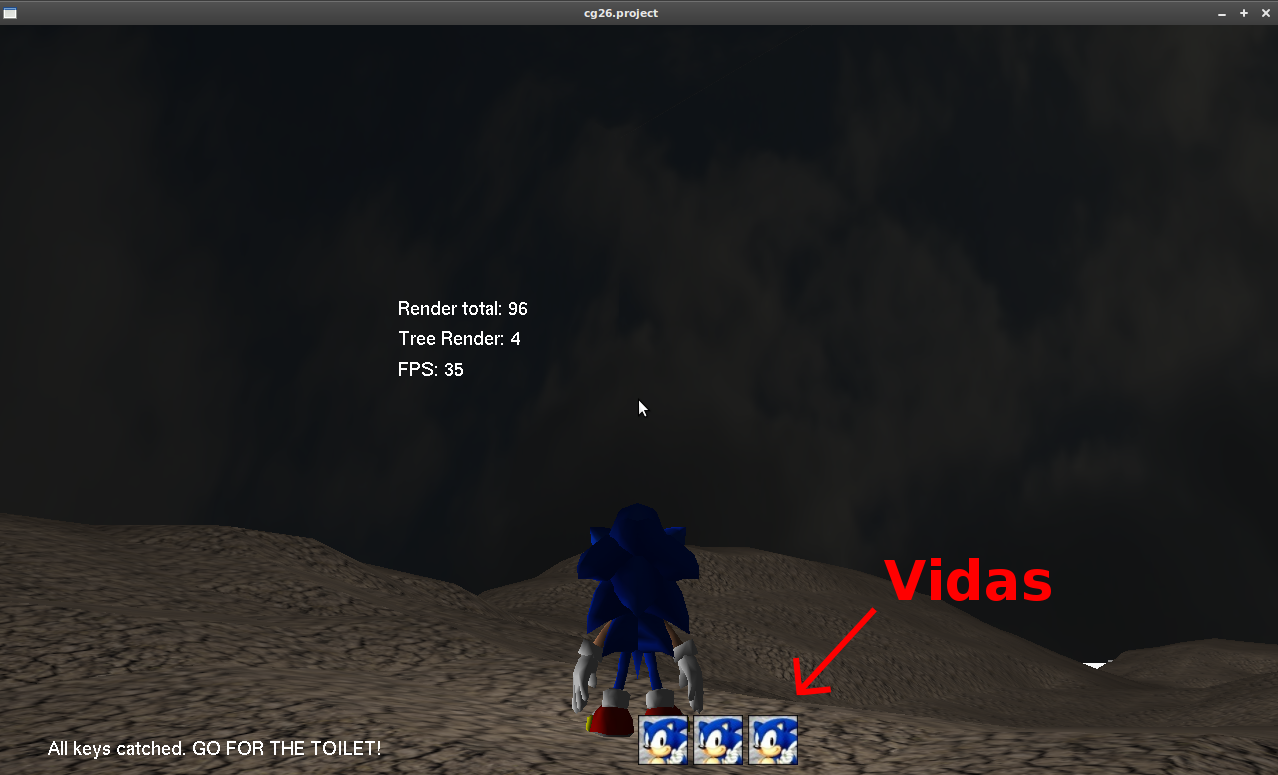
\includegraphics[width=0.8\textwidth]{images/lifes.png}}
                 \caption{Screenshot para as vidas.}
                 \label{fig:prototype}
\end{figure}


\section{Colisões}
\section{Salto}

Apenas a experiência terá algo a acrescentar. Terminamos assim com algo cuja imagem fala por si, um conceito simples, aos requisitos acrescentamos as árvores, de referir também as colisões com árvores e torres, a possibilidade de saltar, e assim evitar as balas, o céu, as animações, as imagem das vidas, o full screen, isto, em termos de jogo, em termos de implementação contamos com o documento de configuração \textit{.ini}, o md2loader, profilling, entre outros.

%\input{7acron}

\appendix
\chapter{Código fonte}
%\section*{Model.h}
\lstinputlisting{../Model.h}
\pagebreak
\section*{GLManager.cpp}
\lstinputlisting{../GLManager.cpp}
\pagebreak
\section*{Config.cpp}
\lstinputlisting{../Config.cpp}
\pagebreak
\section*{SkyBox.cpp}
\lstinputlisting{../SkyBox.cpp}
\pagebreak
\section*{Towers.h}
\lstinputlisting{../Towers.h}
\pagebreak
\section*{Bullet.h}
\lstinputlisting{../Bullet.h}
\pagebreak
\section*{Vertex.h}
\lstinputlisting{../Vertex.h}
\pagebreak
\section*{Key.h}
\lstinputlisting{../Key.h}
\pagebreak
\section*{Model\_MD2.h}
\lstinputlisting{../Model_MD2.h}
\pagebreak
\section*{Sound.h}
\lstinputlisting{../Sound.h}
\pagebreak
\section*{Keys.cpp}
\lstinputlisting{../Keys.cpp}
\pagebreak
\section*{Tower.h}
\lstinputlisting{../Tower.h}
\pagebreak
\section*{Profiling.h}
\lstinputlisting{../Profiling.h}
\pagebreak
\section*{Lifes.h}
\lstinputlisting{../Lifes.h}
\pagebreak
\section*{Player.cpp}
\lstinputlisting{../Player.cpp}
\pagebreak
\section*{Trees.h}
\lstinputlisting{../Trees.h}
\pagebreak
\section*{InputManager.cpp}
\lstinputlisting{../InputManager.cpp}
\pagebreak
\section*{Towers.cpp}
\lstinputlisting{../Towers.cpp}
\pagebreak
\section*{Plane.h}
\lstinputlisting{../Plane.h}
\pagebreak
\section*{Map.cpp}
\lstinputlisting{../Map.cpp}
\pagebreak
\section*{Frustum.cpp}
\lstinputlisting{../Frustum.cpp}
\pagebreak
\section*{Map.h}
\lstinputlisting{../Map.h}
\pagebreak
\section*{SkyBox.h}
\lstinputlisting{../SkyBox.h}
\pagebreak
\section*{InputManager.h}
\lstinputlisting{../InputManager.h}
\pagebreak
\section*{Toilet.h}
\lstinputlisting{../Toilet.h}
\pagebreak
\section*{Bullet.cpp}
\lstinputlisting{../Bullet.cpp}
\pagebreak
\section*{Radar.cpp}
\lstinputlisting{../Radar.cpp}
\pagebreak
\section*{Lighting.h}
\lstinputlisting{../Lighting.h}
\pagebreak
\section*{Lifes.cpp}
\lstinputlisting{../Lifes.cpp}
\pagebreak
\section*{ChangeMode.h}
\lstinputlisting{../ChangeMode.h}
\pagebreak
\section*{Lighting.cpp}
\lstinputlisting{../Lighting.cpp}
\pagebreak
\section*{Rainbow.h}
\lstinputlisting{../Rainbow.h}
\pagebreak
\section*{Player.h}
\lstinputlisting{../Player.h}
\pagebreak
\section*{Frame.h}
\lstinputlisting{../Frame.h}
\pagebreak
\section*{Trees.cpp}
\lstinputlisting{../Trees.cpp}
\pagebreak
\section*{Config.h}
\lstinputlisting{../Config.h}
\pagebreak
\section*{Textures.cpp}
\lstinputlisting{../Textures.cpp}
\pagebreak
\section*{externs.h}
\lstinputlisting{../externs.h}
\pagebreak
\section*{Rainbow.cpp}
\lstinputlisting{../Rainbow.cpp}
\pagebreak
\section*{Bullets.h}
\lstinputlisting{../Bullets.h}
\pagebreak
\section*{Textures.h}
\lstinputlisting{../Textures.h}
\pagebreak
\section*{Sound.cpp}
\lstinputlisting{../Sound.cpp}
\pagebreak
\section*{Radar.h}
\lstinputlisting{../Radar.h}
\pagebreak
\section*{Tree.cpp}
\lstinputlisting{../Tree.cpp}
\pagebreak
\section*{Key.cpp}
\lstinputlisting{../Key.cpp}
\pagebreak
\section*{Model\_MD2.cpp}
\lstinputlisting{../Model_MD2.cpp}
\pagebreak
\section*{Model.cpp}
\lstinputlisting{../Model.cpp}
\pagebreak
\section*{Tree.h}
\lstinputlisting{../Tree.h}
\pagebreak
\section*{GLManager.h}
\lstinputlisting{../GLManager.h}
\pagebreak
\section*{Camera.cpp}
\lstinputlisting{../Camera.cpp}
\pagebreak
\section*{Camera.h}
\lstinputlisting{../Camera.h}
\pagebreak
\section*{Frustum.h}
\lstinputlisting{../Frustum.h}
\pagebreak
\section*{Toilet.cpp}
\lstinputlisting{../Toilet.cpp}
\pagebreak
\section*{ChangeMode.cpp}
\lstinputlisting{../ChangeMode.cpp}
\pagebreak
\section*{Profiling.cpp}
\lstinputlisting{../Profiling.cpp}
\pagebreak
\section*{Plane.cpp}
\lstinputlisting{../Plane.cpp}
\pagebreak
\section*{Keys.h}
\lstinputlisting{../Keys.h}
\pagebreak
\section*{Main.cpp}
\lstinputlisting{../Main.cpp}
\pagebreak
\section*{Tower.cpp}
\lstinputlisting{../Tower.cpp}
\pagebreak
\section*{Bullets.cpp}
\lstinputlisting{../Bullets.cpp}
\pagebreak
\section*{Vertex.cpp}
\lstinputlisting{../Vertex.cpp}
\pagebreak
\section*{Frame.cpp}
\lstinputlisting{../Frame.cpp}
\pagebreak

%\input{8anexos}

\end{document}
  